\documentclass{article}
\usepackage{svg}
\usepackage{hyperref}
\usepackage{amsmath}
\usepackage{amsfonts} 
\usepackage{graphicx}
\usepackage{minted}
\usepackage[a4paper,  total={6.75in, 10in}]{geometry}
\usepackage[utf8]{inputenc}


\title{Simulazione di una pandemia con un modello SMRV}
\author{Giulio Pastorello, Federico Gnudi}
\date{Novembre 2023}

\begin{document}

\maketitle

\section{Il Modello}

\hspace{\parindent} Per descrivere l'andamento della pandemia si è scelto 
di usare un modello SIR al quale è stata aggiunta un quarta 
equazione per rappresentare i vaccinati.\\
Le equazioni che descrivono l'evoluzione della pandemia sono quindi:
\begin{itemize}
\item $S(t)$: "Suscettibili". Descrive il numero delle persone non 
malate che non hanno mai contratto l'infezione.
\item $M(t)$: "Malati". Il numero di persone che ad un dato tempo 
t sono malate. 
\item $R(t)$: "Rimossi". Una volta che una persona è stata 
contagiata, dopo un certo intervallo di tempo viene \textit{rimossa}, 
ovvero guarisce o muore. Si assume che, una volta guariti, 
i soggetti diventino immuni. L'unica possibilità di transizione da 
uno stato all'altro è quindi: $S\xrightarrow{}I\xrightarrow{}R$.
\item $V(t)$: "Vaccinati". Questa equazione è un'aggiunta al modello 
SIR "standard", che prevede solo le prime tre equazioni. 
Anche in questo caso si fa l'assunzione che una persona vaccinata 
non possa più ammalarsi.
\end{itemize}
Il vincolo fondamentale del modello è che la popolazione totale 
sia costante:
\begin{equation}\label{eq::pop}
S(t)+M(t)+R(t)+V(t)=N
\end{equation}
Questa è un'approssimazione ragionevole se si fa l'assunzione 
che il numero totale di persone che muoiono a causa del virus 
sia trascurabile rispetto alla popolazione totale. 
\subsection{Parametri}
Il modello descrive l'andamento della pandemia attraverso alcuni 
parametri:
\begin{itemize} 
\item $\beta \in [0,1]$: questo è interpretabile come la 
\textit{contagiosità} del virus, ovvero la probabilità di 
trasmissione a seguito di un contatto tra un suscettibile e un infetto.
\item $\gamma \in [0,1]$: è l'inverso della durata media di 
un'infezione, che corrisponde alla probabilità di guarigione o morte.
\item $\eta \in \mathbb{N}, \eta < N$: il numero di persone non 
vaccinabili, per motivi medici o personali. Nel caso in cui 
$\eta = N$ semplicemente si ha il modello SIR, però a causa della 
forma dell'equazione scelta, il valore $N$ non è accettabile.
\item $\mu \in [0,1]$: rappresenta la velocità delle vaccinazioni.
\item $\xi \in [0,1]$: rappresenta l'efficacia delle vaccinazioni. 
Si usa come fattore moltiplicativo.
\end{itemize}

\subsection{Condizioni Iniziali}
Per studiare la diffusione del virus vengono anche usati come 
condizioni iniziali i seguenti termini:
\begin{itemize}
\item $S_0 \in \mathbb{N}$: suscettibili al tempo $t = 0$.
\item $M_0 \in \mathbb{N}$: malati al tempo $t = 0$.
\item $R_0 \in \mathbb{N}$: rimossi al tempo $t = 0$.
\item $V_0 \in \mathbb{N}$: vaccinati al tempo $t = 0$.
\end{itemize}
Ovviamente si avrà che la popolazione totale sarà: 
$$N = S_0 + M_0 + R_0 + V_0$$.\\
\subsection{Equazioni}
Usando i parametri descritti sopra, le equazioni differenziali che 
descrivono la diffusione della pandemia sono quindi quattro:\\
\begin{equation} \label{eq::S}
\frac{dS}{dt}(t)= -\beta \frac{S(t)}{N}M(t) - \frac{dV}{dt}(t)
\end{equation}
\begin{equation}\label{eq::M}
\frac{dM}{dt}(t)= \beta \frac{S(t)}{N}M(t) - \gamma I(t)
\end{equation}
\begin{equation}\label{eq::R}
\frac{dR}{dt}(t)= \gamma M(t)
\end{equation}
\begin{equation}\label{eq::V}
\frac{dV}{dt}(t)= \mu\frac{V(t)}{\xi}\left( 1-\frac{V(t)}{\xi(N-\eta)}\right)
\end{equation}
Una simulazione basata su dati rappresentativi dell'Emilia-Romagna
realizzata con Wolfram Mathematica è mostrata in figura 
(\ref{fig::SIRV}). 
Si è usato: popolazione totale $N=4459000$, $\beta=0.05$, 
$\gamma=0.02$, $M_0 = 530502$, $R_0 = 320000$, $V_0 = 600437$,
non vaccinabili $\eta = 251042$, 
velocità vaccinazioni $\mu = 0.05$, efficacia 
vaccino $\xi= 0.83$.

\subsection{Curva Logistica}
Per rappresentare la progressione della campagna vaccinale, 
nell'equazione (\ref{eq::V}) si è scelto di usare un'equazione 
logistica generalizzata: $f'(x)=f(x)(1-f(x))$,
che ha come soluzione un sigmoide. Quest'approssimazione è 
ragionevole perché ci si aspettava un inizio più lento dovuto alla 
scarsità di vaccini e all'organizzazione non ancora rodata, 
seguito da una crescita veloce della quantità di persone vaccinate, 
seguito inevitabilmente da una diminuzione dovuta al fatto che le 
persone da vaccinare sono sempre meno. 
Il limite dell'equazione logistica è che usando come numero di 
vaccinati iniziali $V_0  = 0$ la campagna vaccinale resta a zero, 
ma partendo da un qualsiasi altro numero si arriverà sicuramente a 
vaccinare tutti i vaccinabili, in un tempo che dipende dalla velocità 
delle vaccinazioni $\mu$. In figura (\ref{fig::vaccinati}) un 
andamento possibile della curva dei vaccinati.\\
\begin{figure}[h!]
\centering
\begin{minipage}[t]{.4\paperwidth}
    \hspace{-10pt}
    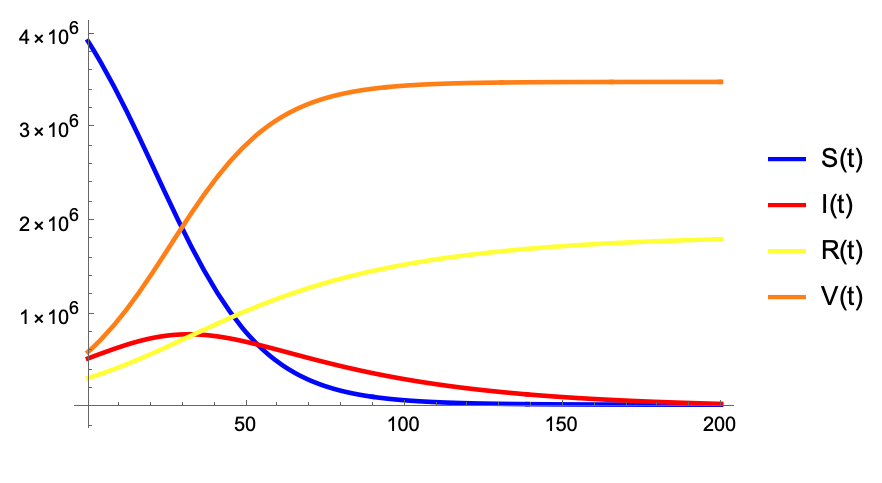
\includegraphics[width=\textwidth]{SIRV.png}
    \caption{\textit{Comportamento del modello SIRV con dati 
    rappresentativi dell'Emilia-Romagna}}
    \label{fig::SIRV}
    \end{minipage}%
\hfill %
\begin{minipage}[t]{.4\paperwidth}
    \hspace{-10pt}
    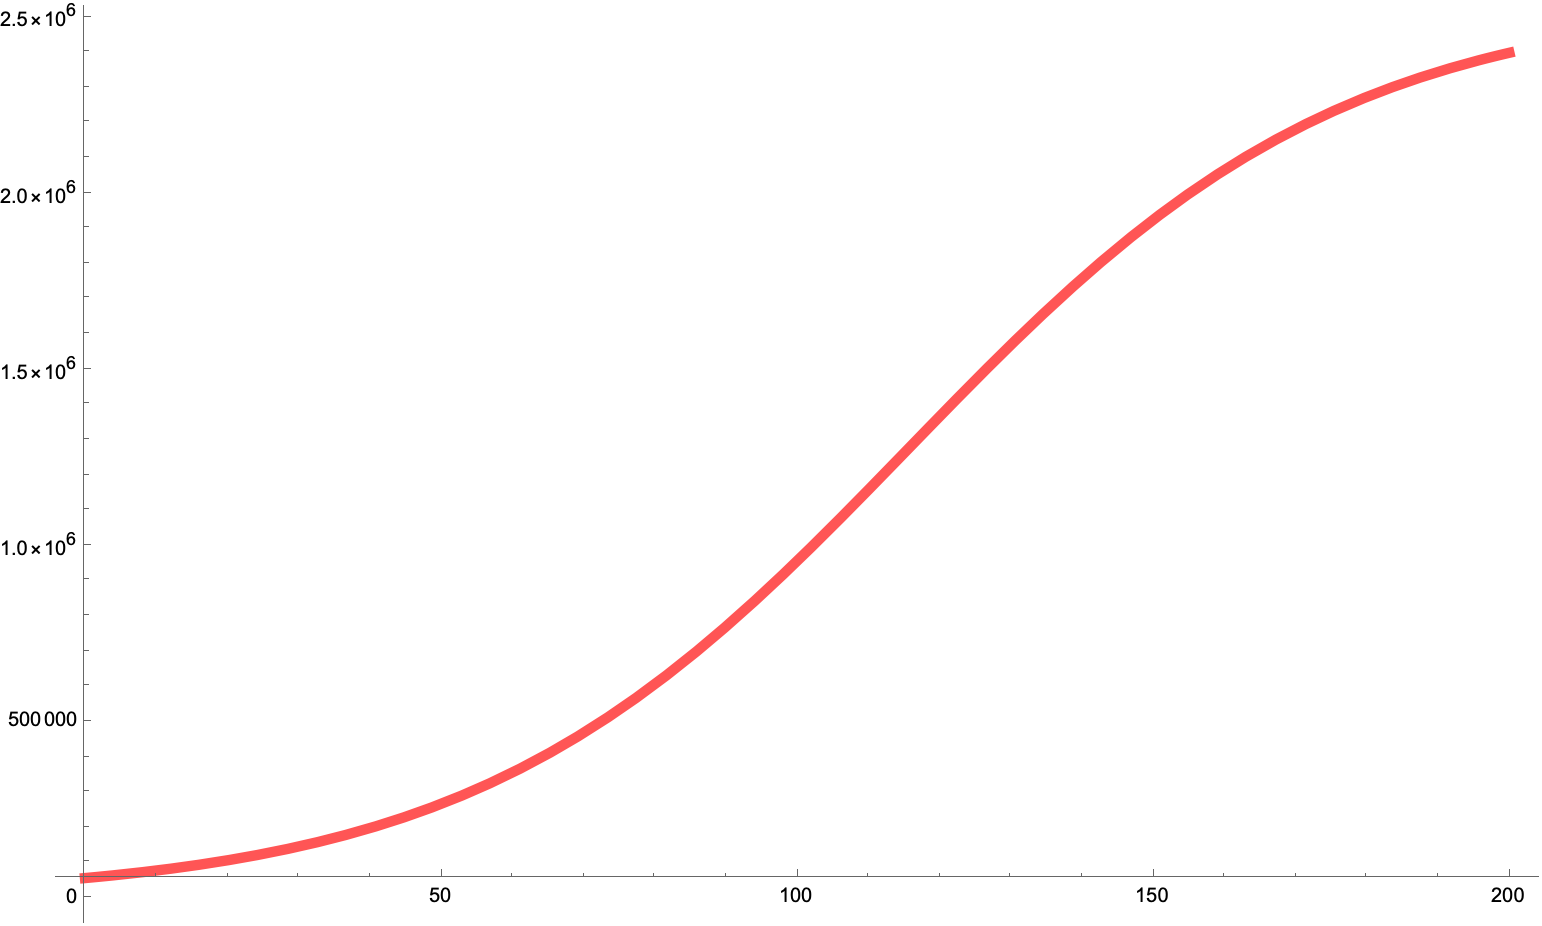
\includegraphics[width=\textwidth]{vaccinati.png}
    \caption{\textit{Curva logistica con $\nu=56980, 
    \mu=0.0274216, \eta=1418957$, e popolazione totale della regione 
    Emilia-Romagna.}}
    \label{fig::vaccinati}
\end{minipage}
\end{figure}

\section{I Metodi Numerici}

\hspace{\parindent} Per calcolare i risultati prodotti dal modello 
si sono scritti due diversi metodi numerici: il \textit{metodo di Eulero},
meno preciso ma anche meno dispendioso a livello di calcoli, e il 
metodo \textit{Runge-Kutta 4}, che è più complesso ma produce 
risultati migliori.

\subsection{Il metodo di Eulero}
Il metodo di Eulero è eseguito dalla funzione \verb|euler()| in 
\verb|infection.cpp|. Dato un probelma di Cauchy nella forma
\begin{equation} \label{eq::ODE} 
    \dot{\vec{x}} = f(t, \vec{x}), \qquad \vec{x}(t_0) = \vec{x_0}
\end{equation}
con $f(t, \vec{x})$ campo vettoriale che descrive il sistema di 
equazioni, $\vec{x} \in \mathbb{R}^n$ variabile di stato, 
t variabile indipendente (tempo), e $\vec{x}(t_0) = \vec{x_0}$
condizione iniziale, il \textit{metodo di Eulero} discretizza il 
sistema nella seguente maniera:
\begin{equation} \label{eq::Euler}
    \vec{x}(t_{n+1})=\vec{x}(t_n) + h f(t_n, \vec{x}(t_n))
\end{equation}
dove h è lo \textit{step size}, un intervallo di tempo arbitrario che 
ovviamente determina la precisione dei risultati ottenuti. 
Nel caso dell'\textit{algoritmo di Eulero}, si dimostra che l'errore 
totale è dell'ordine di $O(h^2)$. \\
Nel caso del modello SMRV, il sistema è \textit{autonomo}, ovvero le 
euqazioni non dipendono esplicitamente dal tempo. L'algoritmo di 
discretizzazione assume quindi la forma: 
\begin{equation} \label{eq::autoEuler}
    \vec{x}(t_{n+1})=\vec{x}(t_n) + h f(\vec{x}(t_n))
\end{equation}
Le equazioni risultanti sono i valori che stampiamo:
\begin{equation}\label{eq::euler}
    \left\{ \arraycolsep=1.4pt\def\arraystretch{2.2}
    \begin{array}{rcl}
    S(t_{n+1}) & = & S(t_n) + h \left(-\beta \frac{S(t_n)}{N} M(t_n)
            -\Delta V \right) \\
    M(t_{n+1}) & = & M(t_n)+h\left(\beta \frac{S(t_n)}{N} M(t_n) 
            - \gamma M(t_n)\right) \\
    R(t_{n+1}) & = & R(t_n) + h \gamma M(t_n) \\
    V(t_{n+1}) & = & V(t_n) +h \mu \frac{V(t_n)}{\xi} \left(
            1 - \frac{V(t_n)}{\xi (N - \eta)} \right) \\
    \end{array}\right.
\end{equation}
dove si è usata la notazione $\Delta V = V(t_{n+1})-V(t_n)$. 

\subsection{Runge-Kutta 4th Order}
L'algoritmo alternativo usato per calcolare i valori delle variabili di 
stato giorno-per-giorno è il Runge-Kutta del quarto ordine, abbreviato 
spesso come RK o RK4, che è eseguito nella funzione \verb|rk()| in 
\verb|rk.cpp|.
Come da nome, l'errore totale è dell'ordine di $O(h^4)$.
Partendo da un'equazione generica nella forma dell' eq. (\ref{eq::ODE})
l'approssimazione che viene fatta è la seguente: \\
\begin{equation} \label{eq::rk4}
    \vec{x}(t_{n+1})=\vec{x}(t_n)+\frac{h}{6}(k_1+k_2+k_3+k_4), \qquad
    \left\{ \arraycolsep=1.4pt\def\arraystretch{2.2}
    \begin{array}{rcl}
    k_1 & = & f(t_n, \vec{x}(t_n)) \\
    k_2 & = & f(t_n+\frac{h}{2}, \vec{x}(t_n)+h\frac{k_1}{2}) \\
    k_3 & = & f(t_n+\frac{h}{2}, \vec{x}(t_n)+h\frac{k_2}{2}) \\
    k_4 & = & f(t_n+h, \vec{x}(t_n)+hk_3) \\
    \end{array}\right.
\end{equation}
Nel caso del nostro modello, ricordando che il sistema è autonomo (ovvero
il campo è nella forma $f(\vec{x})$), il calcolo dei coefficienti è dato 
dalle seguenti espressioni:
\begin{equation} \label{eq::rk4Coeff}
    \left\{ \arraycolsep=1.4pt\def\arraystretch{2.2}
    \begin{array}{crcl}
    (V) & a_1 & = & \mu \frac{V(t)}{\xi}\left(1-\frac{V(t)}
    {\xi(N-\eta)}\right) \\
    (S) & b_1 & = &  -\beta\frac{S(t)}{N}M(t)-a_1\\
    (R) & c_1 & = &  \gamma M(t)\\
    (M) & d_1 & = &  -a_1-b_1-c_1 \\
    \end{array}\right. \quad
    \left\{ \arraycolsep=1.4pt\def\arraystretch{2.2}
    \begin{array}{rcl}
    a_2 & = & \mu \frac{V(t) + a_1 h/2}{\xi}\left(1-\frac{V(t)+
    a_1 h/2}{\xi(N-\eta)}\right) \\
    b_2 & = &  -\beta\frac{S(t)+b_1 h/2}{N}(M(t)+d_1 h/2)-a_2\\
    c_2 & = &  \gamma (M(t)+d_1 h/2)\\
    d_2 & = &  -a_2-b_2-c_2 \\
    \end{array}\right. \quad ...
\end{equation}
Scegliendo lo step size $h=1$(giorno), si otterranno i valori delle 
quattro variabili di ogni giorno. Ad ogni iterazione vengono ri-calcolati
i coefficienti $a_i, b_i, c_i,d_i, i \in \{1,2,3,4\}$, che sarebbero dunque
16 valori per ogni giornata. Sfruttando il fatto che c'è un vincolo sulla
popolazione totale, si riesce a esprimere uno dei quattro coefficienti 
in funzione degli altri  tre, e quindi i valori da calcolare si riducono 
a 12 per ogni giornata.\\
\section{Il Codice}
\hspace{\parindent} Si è diviso il codice in più 
\textit{translation units}: \verb|infection.cpp|,
\verb|display.cpp| e \verb|main.cpp|. Di seguito si dà una una breve 
spiegazione del funzionamento e dei metodi implementati.
\subsection{Infection}
\subsubsection{La classe}
Per rendere il codice più leggibile si è scelto di raccogliere i metodi
riguardanti l'evoluzione della pandemia all'interno del 
\mint{C++}|namespace epidemic{.|
All'interno di \verb|infection.h| si è definita una struct 
\verb|State|: 
\begin{minted}{C++}
    struct State {
        int S; 
        int M; 
        int R; 
        int V; 
      };
\end{minted}
che descrive i valori delle quattro variabili di stato in un dato giorno.
Si è poi scritta la classe \verb|Infection|
\begin{minted}{C++}
    class Infection {

    int m_time_indays; 
    std::vector<State> m_data; 
    int m_N; 
\end{minted}    
che ha come membri privati la durata della simulazione, un vettore di 
stati, che rappresenta l'evoluzione della pandemia, e la popolazione 
totale.
\subsubsection{Evoluzione}
Come anticipato sopra, si può scegliere fra due diversi metodi 
numerici per discretizzare le equazioni del modello.\\
Il primo è il metodo di Eulero, implementato dal metodo 
\verb|euler()|:
\begin{minted}{C++}
    Infection euler(Infection const &plague, double beta, 
    double gamma, int no_vax, double vel_vax, double eff_vax) {
\end{minted}
Come descritto sopra, nel metodo evolve non si riesce a sfruttare
il vincolo della popolazione totale, in quanto la precisione troppo
bassa produce risultati troppo lontani dalla soluzione ideale.
Si calcolano le 4 pendenze per ogni giornata, e poi tramite un 
assert
\mint{C++}|assert(support.M + support.R + support.S + support.V == result.get_N());|
ci si assicura che la popolazione totale resti costante, aggiungendo
o sottraendo al numero dei suscettibili in caso contrario.
questa scelta è stata fatta poiché in una simulazione realistica
il numero dei suscettibili sarà sempre molto maggiore degli altri.\\
L'altra opzione proposta è il metodo Runge-Kutta in \verb|RK4()|:
\begin{minted}{C++}
    Infection RK4(Infection const &plague, double beta, 
    double gamma, int no_vax, double vel_vax, double eff_vax) {
\end{minted}
Qui invece si è potuta sfruttare l'esistenza di un integrale primo
per semplificare i calcoli. Si è infatti verificato che i risultati 
prodotti calcolando tutte e quattro le pendenze o solamente tre erano
pressoché identici (per simulazioni con numeri realistici).
Anche in questo metodo viene sempre controllato che N resti 
costante e in caso contrario vengono aggiunti/rimossi suscettibili 
finché la condizione non è soddisfatta.
\subsubsection{Display}
In \verb|display.cpp| si sono raggruppati i metodi che, come da 
nome, danno una rappresentazione dei risultati ottenuti.\\
Il primo metodo è 
\mint{C++}|void print(Infection const &infection){|
che stampa sul terminale i risultati della simulazione e il valore 
\verb|int| del giorno, avvalendosi della funzione 
\mint{C++}|int count_digit(int n){|
dichiarata sempre all'interno di \verb|display.hpp|, che serve ad 
impaginare in modo leggibile i valori stampati.
Si è usata inoltre la libreria \verb|termcolor| che permette di 
colorare quanto stampato su terminale per distinguere meglio
i nomi delle variabili. \\
Oltre a stampare i valori della simulazione su terminale si è voluto
scrivere un metodo che facesse degli istogrammi per rappresentare i
valori delle variabili giorno-per-giorno.
Questa funzione è implementata dal metodo \verb|graph()|:
\mint{C++}|void graph(Infection const &infection) {|
Per questo si è usata la libreria \verb|matplotplusplus|, che è 
basata su \verb|gnuplot|. Al \textit{run-time} viene protto un 
file contenente i quattro istogrammi che viene salvato 
automaticamente in formato .jpg e viene sovrascritto ogni volta che
viene fatto girare di nuovo il programma.
\subsubsection{Main}
Viene proposto all'utente di cambiare i valori di default di 
parametri e valori iniziali, che sono stati scelti per essere 
rappresentativi della situazione in Emilia-Romagna nel'estate del 
2021. Si può anche cambiare la durata della simulazione, 
pre-impostata a 100 giorni.
Una volta fatta questa scelta, l'utente può scegliere quale metodo 
numerico usare per la simulazione. A questo punto vengono stampati 
su terminale i valori delle quattro variabili giorno-per-giorno e 
viene prodotto il file .jpg con gli istogrammi.
\section{Compilazione}
\hspace{\parindent} Per costruire il programma si è deciso di usare 
\verb|cmake|, nel folder \verb|parte1/| è incluso il 
\verb|CMakeLists.txt| che permette di costruire il progetto 
(caricando la libreria di plotting).\\
Per compilare serve fare la build con :
\begin{minted}{C++}
    cmake .  
    cmake --build .
\end{minted} 
Una volta fatto questo vengono prodotti due
eseguibili: \verb|infection_tty| e \verb|infection.test|.
Poiché la libreria \verb|matplotplusplus| dava alcuni problemi di
linking su MacOS, si è deciso semplicemente di clonare la repository
github della libreria all'interno del folder in cui viene implementata, 
utilizzando il comando \verb|add_subdirectory(matplotplusplus)|
di CMake.
\subsection{Come compilare}
Per il progetto è necessario avere:
\begin{itemize}
    \item \verb|cmake| versione 16 o superiore;
    \item la libreria \verb|matplotplusplus|. Basta clonare la 
    \href{https://github.com/alandefreitas/matplotplusplus}{repository 
    github} della libreria all'interno del
    folder \verb|parte1/|. 
    \item la libreria \verb|gnuplot|. Seguire le istruzioni sul 
    \href{http://www.gnuplot.info}{sito} della libreria.
\end{itemize}
\section{Appendice}
\subsubsection{Git e Github}
Durante la realizzazione del progetto è stato fondamentale l'uso di 
Github per coordinare i lavori. Si lascia il 
\href{https://github.com/giuliopastorello/progetto_SMRV}{link} alla 
repository remota qualora potesse servire. Per usare il progetto senza
clonare la libreria di plotting si può semplicemente clonare la 
remote repository.
\subsubsection{Nome del modello}
Per testare se il modello avesse senso, prima di cominciare a scrivere
il codice, si è usato Wolfram Mathematica per testare alcune 
possibilità. Su Mathematica I è un carattere riservato, e quindi si 
è dovuto usare un'altra lettere. La scelta della M per descrivere i 
malati era ragionevole, e il nome è rimasto invariato anche quando
si è scritto il programma presentato.
\subsubsection{Risorse}
\begin{itemize}
    \item cmake: \href{https://cmake.org/}{https://cmake.org/}
    \item matplotplusplus : \href{https://github.com/alandefreitas/matplotplusplus}{https://github.com/alandefreitas/matplotplusplus}
    \item gnuplot: \href{http://www.gnuplot.info}{http://www.gnuplot.info}
    \item github: \href{https://github.com/giuliopastorello/progetto_SMRV}{https://github.com/giuliopastorello/progettoSMRV}
\end{itemize}    
\end{document}
